\documentclass{article}
\usepackage{tikz, comment}
\usepackage{pifont}
\usepackage{fontspec, pgfplots}
\usetikzlibrary{arrows, decorations.markings, decorations.pathreplacing}
\begin{comment}
:Title: Not defined yet
:Tags: focal radius ;end behavior;triangle inequality;origin;perimeter
:Prob: 0.511;0.5097;0.5011;0.4952;0.4812
:Author: Prof.Hu Ji-shan, HKUST
:Slug: No name yet

Description Here.........
\end{comment}
\begin{document}\centering 

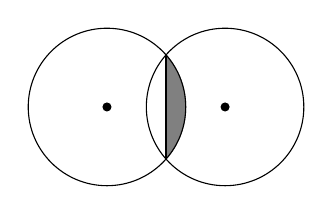
\begin{tikzpicture}[>=latex,xscale=.5*1, yscale=.5*1][font=\sf\small] 

%\draw[xstep=1cm,ystep=1cm,color=gray!80] (0, -1) grid (8, 8);

\draw[gray, fill, samples=100, smooth, domain=-0.722734:0.722734, variable=\x] 
		plot ({2*cos(\x r)}, {2*sin(\x r)}) -- (3/2, {-1*sqrt(7)/2}); 

\draw (0, 0) circle(2); \draw[fill] (0, 0) circle(0.1); 
\draw (3, 0) circle(2); \draw[fill] (3, 0) circle(0.1); 

\draw (3/2, {sqrt(7)/2}) -- (3/2, {-1*sqrt(7)/2});

\end{tikzpicture}
\end{document}